\documentclass[12pt, twoside]{article}
\usepackage[francais]{babel}
\usepackage[T1]{fontenc}
\usepackage[latin1]{inputenc}
\usepackage[left=7mm, right=7mm, top=7mm, bottom=7mm]{geometry}
\usepackage{float}
\usepackage{graphicx}
\usepackage{array}
\usepackage{multirow}
\usepackage{amsmath,amssymb,mathrsfs} 
\usepackage{soul} 
\usepackage{textcomp}
\usepackage{eurosym}
\usepackage{lscape} 
 \usepackage{variations}
\usepackage{tabvar}
  
\pagestyle{empty}

\title{\ul{\textbf{Activit�: th�or�me de Thal�s}}}
\date{} 

\begin{document}
\maketitle




\ul{M�thode pour calculer une longueur}:

\begin{tabular}{cc}
\begin{minipage}{10cm}
Sur la figure ci-contre, les droites (OL) et (TE) sont parall�les. On donne
HE=5cm, HL=2cm, TE=7cm et HO=3cm. Calculer les longueurs HT et OL.

\end{minipage}
&
\begin{minipage}{8cm}
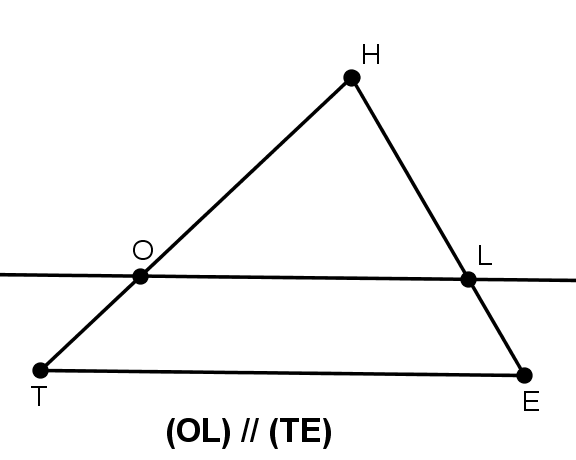
\includegraphics[width=5cm]{images/ex2.png}
\end{minipage}
\end{tabular}


\bigskip



 Dans le triangle \ldots\ldots, on sait que:

\begin{itemize}
  \item [$\bullet$] \ldots \ldots \ldots \ldots \ldots
  \item [$\bullet$] \ldots \ldots \ldots \ldots \ldots
  \item [$\bullet$] \ldots \ldots \ldots \ldots \ldots 
  
\end{itemize}

D'apr�s la propri�t� de proportionnalit� des longueurs dans un triangle, on a:
$\dfrac{\ldots \ldots}{\ldots \ldots}=\dfrac{\ldots \ldots}{\ldots \ldots}=\dfrac{\ldots \ldots}{\ldots \ldots}$.

En rempla�ant par les valeurs num�riques:
$\dfrac{\ldots \ldots}{HT}=\dfrac{\ldots \ldots}{\ldots \ldots}=\dfrac{OL}{\ldots \ldots}$


\enskip

\textbf{Calcul de HT:} 

\enskip

\textbf{Calcul de OL:} 



\bigskip



\bigskip


\textit{Faire l'exercice 4 p 184}


\bigskip


\bigskip

\ul{Une nouvelle configuration: ``configuration papillon''}

\enskip

\begin{tabular}{cc}
\begin{minipage}{11cm}
Sur la figure ci-contre, les droites (BE) et (CF) sont s�cantes au point A et
les droites (BC) et  (EF) sont parall�les.
 
\end{minipage}
&
\begin{minipage}{7cm}
\begin{center}
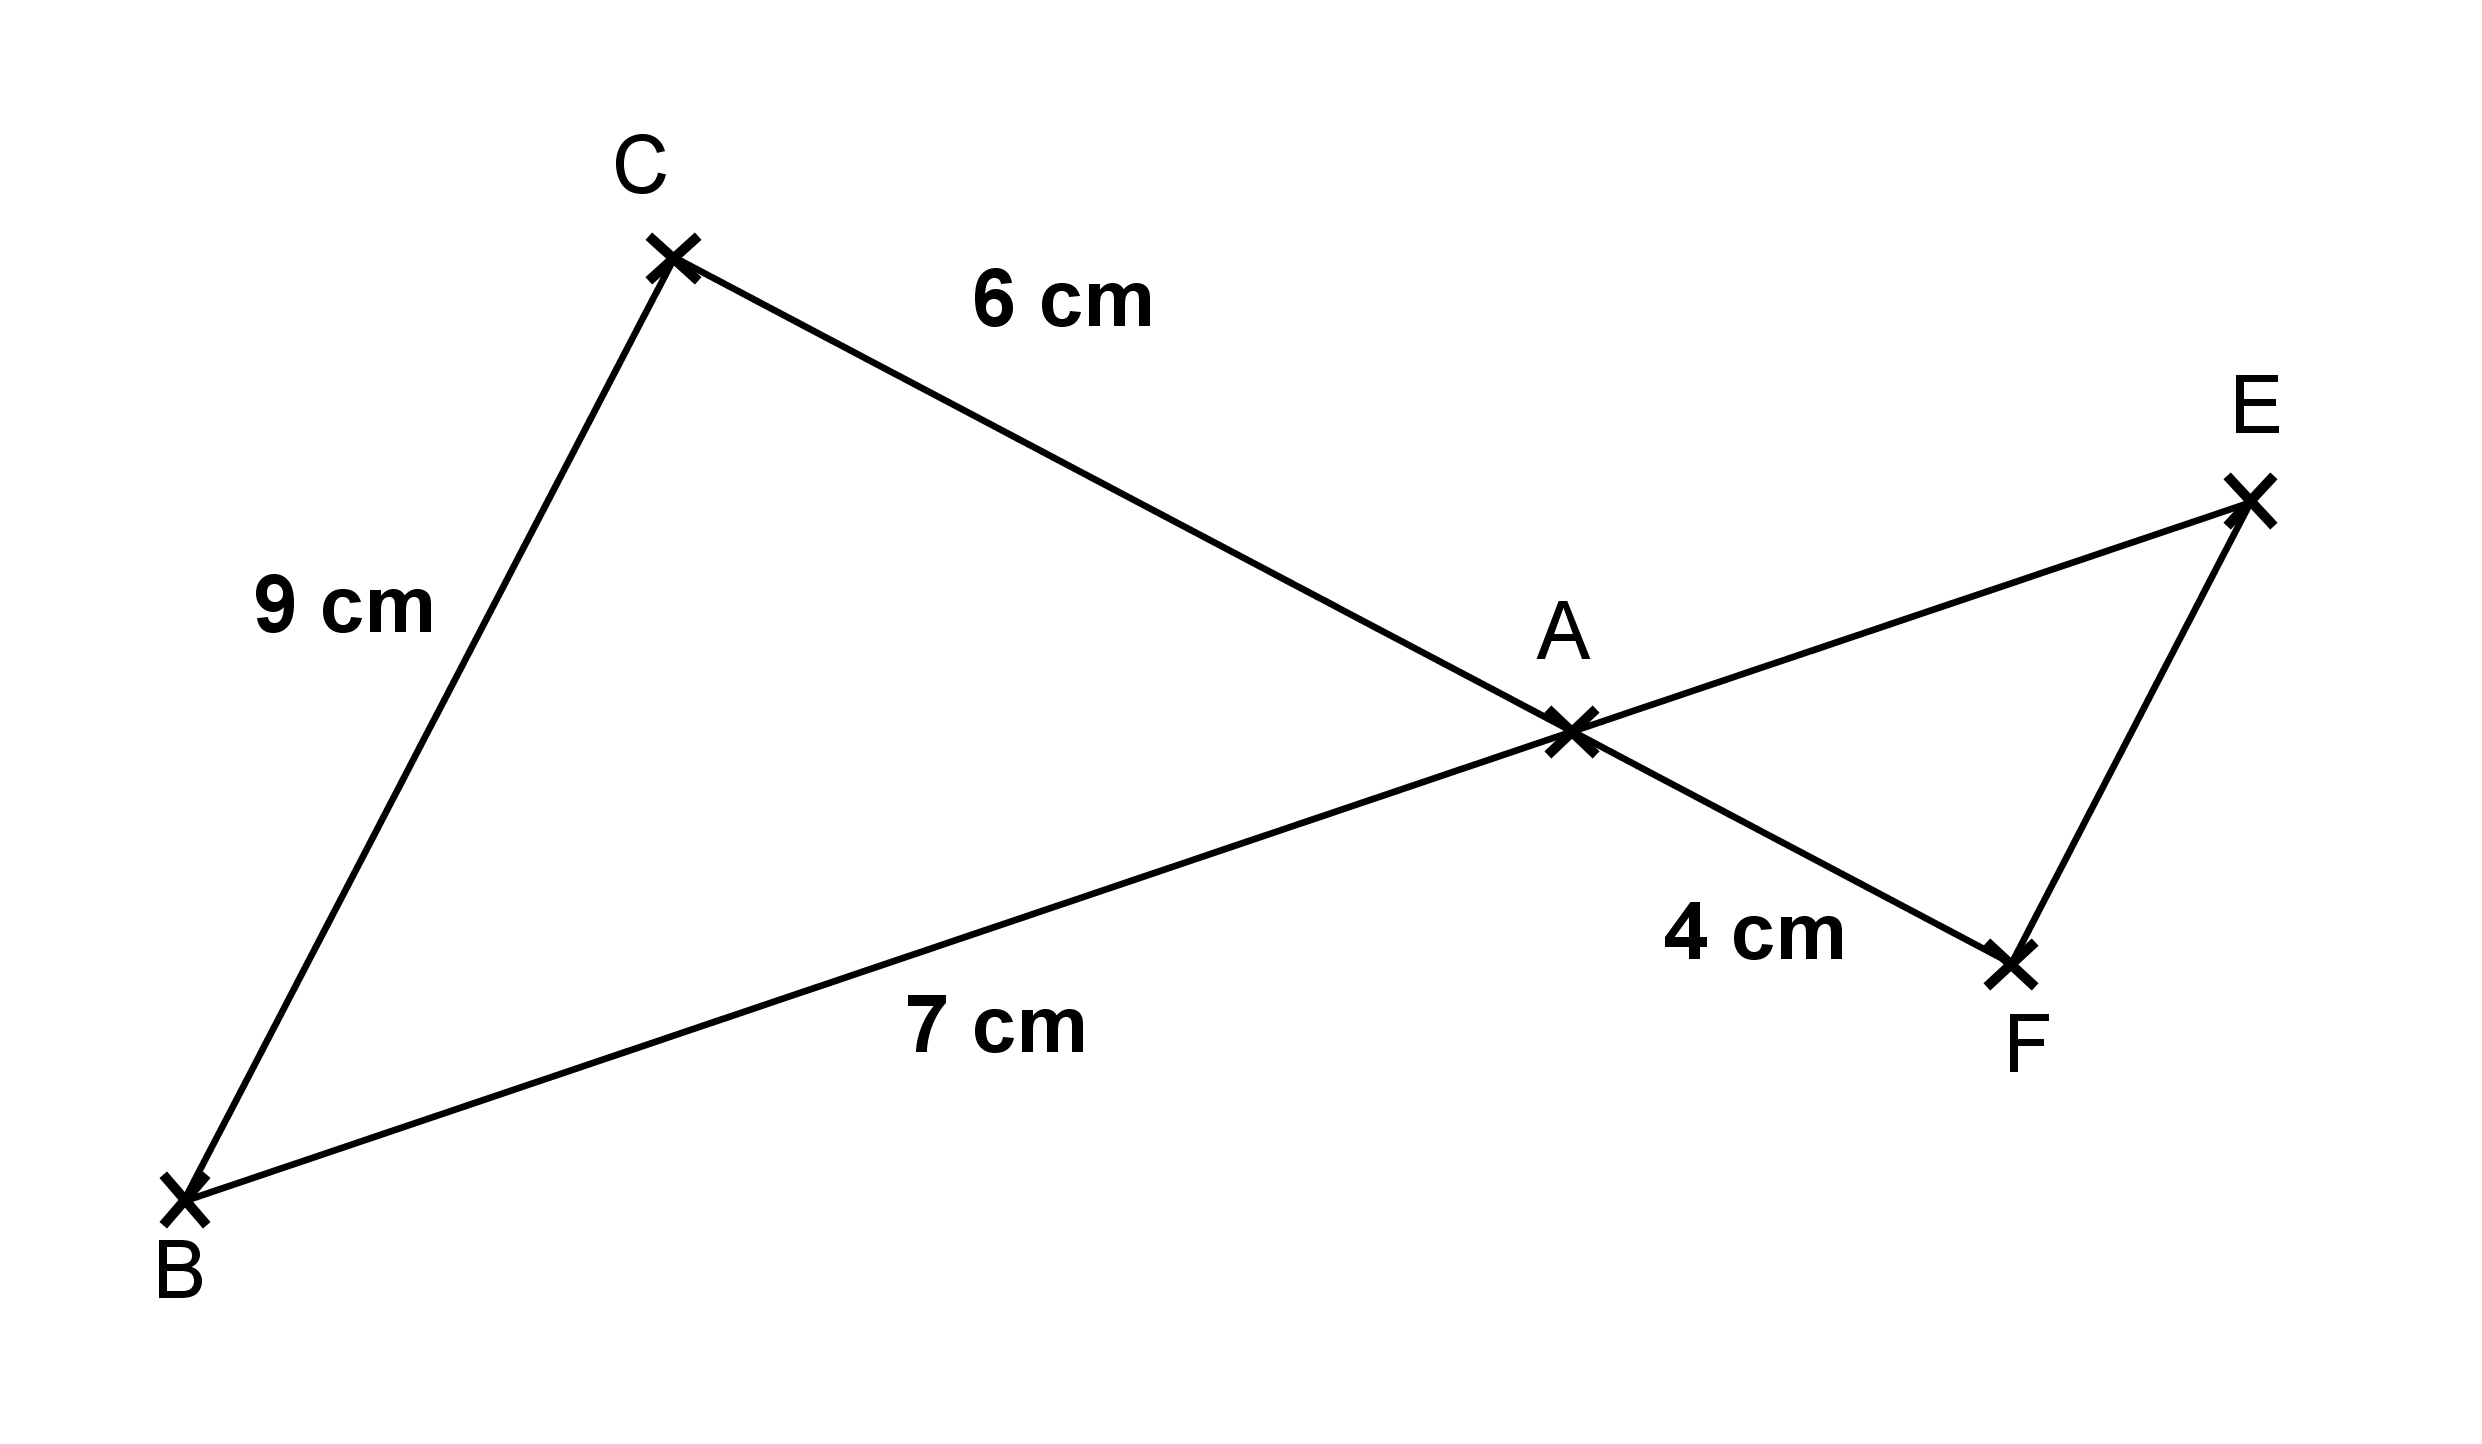
\includegraphics[width=6cm]{images/papillon.png}
\end{center}
\end{minipage}
\end{tabular} 


\begin{enumerate} 
  \item Reproduire en vraie grandeur la figure.
  \item Construire les points E' et F', sym�triques respectifs des points E et
  F par rapport au point A.
  \item Tracer la droite (E'F').
  \item Justifier que les droites (E'F') et (EF) sont parall�les. En d�duire
  que les droites (E'F') et (BC) sont parall�les.
  \item Calculer la longueur E'F' et en d�duire EF.
\end{enumerate}
\end{document}
